% !TeX root = booklet-03.tex
\subsection{مشخصه \lr{DC} یک \lr{Static CMOS Inverter}}
\label{sec:inverter-dc}
هدف این بخش، محاسبه \(V_{\mathrm{out}}\) برای هر
\(V_{\mathrm{in}}\) است. مبنای مدار و تقسیم‌بندی، بخش
\secnum{۲.۵.۱} کتاب و اسلایدهای ۳ تا ۷ است
\cite{weste,dcslides}. ابتدا قراردادهای عمومی ولتاژ و جریان را
می‌نویسیم. استخراج پنج ناحیه با مدل متقارن کتاب انجام می‌شود.

\subsubsection{مدار، فرض‌ها و قرارداد علامت}
\label{sec:inverter-conventions}
در شکل \ref{fig:inverter-circuit}، سورس \lr{nMOS} به زمین و سورس
\lr{pMOS} به \(V_{DD}\) متصل است. گیت‌ها به یک ورودی و درین‌ها
به یک خروجی وصل‌اند. بدنه \lr{nMOS} را به زمین و بدنه
\lr{pMOS} را به تغذیه می‌بندیم. پس اختلاف ولتاژ سورس و بدنه برای
هر دو صفر است و تغییر آستانه ناشی از بایاس بدنه در این مدار ایجاد
نمی‌شود. فرض می‌کنیم \(0\le V_{\mathrm{in}},V_{\mathrm{out}}\le V_{DD}\).
\begin{figure}[!htbp]
\centering
\begin{latin}
\PersianMathDigits
\begin{circuitikz}[scale=1,transform shape]
\draw (3,1.3) node[nmos] (n) {};
\draw (3,3.7) node[pmos] (p) {};
\draw (n.S)--(3,0.3) node[ground] {};
\draw (p.S)--(3,4.7) node[ocirc] {} node[above] {\(V_{DD}\)};
\draw (n.D)--(p.D);
\draw (n.G)--(1.3,1.3)--(1.3,3.7)--(p.G);
\draw (1.3,2.5) node[circ] {}--(0.4,2.5) node[ocirc] {}
 node[left] {\(V_{\mathrm{in}}\)};
\draw (3,2.5) node[circ] {}--(5,2.5) node[ocirc] {}
 node[right] {\(V_{\mathrm{out}}\)};
\draw[->] (4.8,4.2)--(4.8,3.3) node[midway,right] {\(I_p\)};
\draw[->] (4.8,1.8)--(4.8,0.9) node[midway,right] {\(I_n\)};
\node[right] at (3.3,3.7) {pMOS};
\node[right] at (3.3,1.3) {nMOS};
\end{circuitikz}
\end{latin}
\caption{بازترسیم آموزشی مدار شکل \secnum{۲.۲۵} کتاب و اسلاید ۳.
پیکان‌ها بزرگی جریان‌های بالاکش و پایین‌کش را نشان می‌دهند.
بدنه‌ها به سورس‌های متناظر متصل‌اند.}
\label{fig:inverter-circuit}
\end{figure}

با تعریف اختلاف ولتاژ پایانه‌ها، روابط \lr{nMOS} چنین‌اند
\begin{equation}
 V_{GS,n}=V_{\mathrm{in}},\qquad
 V_{DS,n}=V_{\mathrm{out}}.
 \label{eq:inverter-n-voltages}
\end{equation}
برای \lr{pMOS}، قرارداد علامت‌دار کتاب و قرارداد بزرگی مثبت به‌ترتیب
به صورت زیر به هم مربوط‌اند
\begin{align}
 V_{GS,p}&=V_{\mathrm{in}}-V_{DD},&
 V_{DS,p}&=V_{\mathrm{out}}-V_{DD},
 \label{eq:inverter-p-signed}\\
 V_{SG,p}&=V_{DD}-V_{\mathrm{in}}=-V_{GS,p},&
 V_{SD,p}&=V_{DD}-V_{\mathrm{out}}=-V_{DS,p}.
 \label{eq:inverter-p-magnitudes}
\end{align}
آستانه \lr{nMOS} را \(V_{tn}>0\) و آستانه علامت‌دار
\lr{pMOS} را \(V_{tp}<0\) می‌نامیم. بزرگی آستانه را به صورت زیر
تعریف می‌کنیم.
\[
 V_{TP}=|V_{tp}|=-V_{tp},\qquad V_{TP}>0.
\]
برای جریان نیز
\(I_n=I_{DS,n}\ge0\) و \(I_p=|I_{DS,p}|\ge0\) به کار می‌روند.
با جهت جریان درین به سورس، \(I_{DS,p}=-I_p\) است.

خروجی را بدون جریان بار \lr{DC} فرض می‌کنیم. در حالت ماندگار،
\lr{KCL} به رابطه اصلی تحلیل می‌انجامد
\begin{equation}
 \boxed{I_n(V_{\mathrm{in}},V_{\mathrm{out}})
       =I_p(V_{\mathrm{in}},V_{\mathrm{out}})}.
 \label{eq:inverter-kcl}
\end{equation}
جریان تغذیه در این مدل همان \(I_{DD}=I_p=I_n\) است. وجود ظرفیت
خروجی با این شرط ماندگار سازگار است. اگر بار جریان ثابت یا مقاومتی
داشته باشد، باید \(I_L\) را در معادله گره وارد کرد.

برای استخراج اصلی، فرض‌های متقارن کتاب را به کار می‌بریم
\begin{equation}
 V_{tn}=V_{TP}=V_t>0,\qquad
 \beta_n=\beta_p=\beta>0,\qquad V_{DD}>2V_t.
 \label{eq:inverter-symmetry}
\end{equation}
مدل، \lr{Long-channel Shockley} با آستانه و \lr{Mobility} ثابت است.
در استخراج ایده‌آل، \lr{CLM} و نشتی صفر فرض می‌شوند. شرط آخر،
بازه‌ای برای روشن‌بودن هم‌زمان دو افزاره ایجاد می‌کند. اگر تغذیه
از مجموع بزرگی دو آستانه کمتر باشد، ترتیب پنج‌ناحیه‌ای حاضر
نیازمند بازنگری است و جریان زیرآستانه نیز می‌تواند تعیین‌کننده شود.

پارامتر \(\beta\) با واحد \(\unit{\ampere\per\volt\squared}\)
از \(\beta=\mu C_{\mathrm{ox}}W/L\) به دست می‌آید. با
\(C_{\mathrm{ox}}\) و طول یکسان، برابری دو \(\beta\) نیازمند
\(\mu_nW_n=\mu_pW_p\) است. کتاب برای جبران \lr{Mobility}
کمتر حفره‌ها، عرض \lr{pMOS} حدود دو تا سه برابر \lr{nMOS} را در
تقریب این بخش مطرح می‌کند \cite[صفحه ۸۸]{weste}. این نسبت،
تقریب همان بحث است و مقدار دقیق به فناوری و بایاس وابسته است.

\subsubsection{مدل جریان و تبدیل شرط‌های ناحیه کاری}
\label{sec:inverter-regions}
برای خوانایی روابط، اضافه‌ولتاژهای مثبت را تعریف می‌کنیم
\begin{equation}
 a=V_{\mathrm{in}}-V_{tn},\qquad
 b=V_{DD}-V_{\mathrm{in}}-V_{TP},\qquad
 y=V_{\mathrm{out}},\qquad u=V_{DD}-y.
 \label{eq:inverter-ab-definitions}
\end{equation}
کمیت \(u\) افت ولتاژ سورس به درین \lr{pMOS} است. نمادهای
\(a,b\) با واحد ولت‌اند و تنها وقتی مثبت باشند افزاره متناظر
در مدل هدایت قوی روشن است. روابط جریان مدل مربعی کتاب با این
نمادها چنین نوشته می‌شوند
\begin{equation}
 I_n=
 \begin{cases}
 0,&a\le0,\\[2pt]
 \beta_n(ay-y^2/2),&a>0,\quad 0\le y<a,\\[2pt]
 \beta_n a^2/2,&a>0,\quad y\ge a,
 \end{cases}
 \label{eq:inverter-n-current}
\end{equation}
و برای بزرگی جریان \lr{pMOS} داریم
\begin{equation}
 I_p=
 \begin{cases}
 0,&b\le0,\\[2pt]
 \beta_p(bu-u^2/2),&b>0,\quad 0\le u<b,\\[2pt]
 \beta_p b^2/2,&b>0,\quad u\ge b.
 \end{cases}
 \label{eq:inverter-p-current}
\end{equation}
این روابط از مدل بخش \secnum{۲.۲} کتاب با قراردادهای جدول
\secnum{۲.۲} به دست آمده‌اند \cite[صفحات ۶۶ و ۸۸]{weste}.
در مرز \(y=a\) یا \(u=b\)، دو شاخه روشن، جریان یکسانی می‌دهند.
برای نمونه، \(\beta_n[a(a)-a^2/2]=\beta_na^2/2\).
نسبت‌دادن نقطه مرزی به شاخه اشباع، قرارداد این جزوه است.
در آستانه دقیق، جریان ایده‌آل صفر است.

برای \lr{nMOS} روشن، شرط اشباع
\(V_{DS,n}\ge V_{GS,n}-V_{tn}\) مستقیماً می‌دهد
\(y\ge V_{\mathrm{in}}-V_{tn}\).
برای \lr{pMOS} روشن، از بزرگی ولتاژها شروع می‌کنیم
\begin{align}
 V_{SD,p}&\ge V_{SG,p}-V_{TP},\notag\\
 V_{DD}-y&\ge V_{DD}-V_{\mathrm{in}}-V_{TP},\notag\\
 -y&\ge -V_{\mathrm{in}}-V_{TP},\notag\\
 \boxed{y\le V_{\mathrm{in}}+V_{TP}}.
 \label{eq:inverter-p-saturation-condition}
\end{align}
در مرحله آخر، ضرب در منفی یک، جهت نامساوی را عوض کرده است.
با \(V_{TP}=-V_{tp}\)، این شرط برابر
\(y\le V_{\mathrm{in}}-V_{tp}\) در قرارداد کتاب است.
جدول \ref{tab:inverter-device-regions} همه شرط‌ها را جمع می‌کند
\cite[جدول \secnum{۲.۲}]{weste}\cite[اسلایدهای ۵ و ۶]{dcslides}.
\begin{table}[!htbp]
\centering
\small
\caption{شرط‌های ناحیه کاری در مختصات ورودی و خروجی.
در ردیف‌های روشن، شرط روشن‌بودن نیز باید برقرار باشد.}
\label{tab:inverter-device-regions}
\begin{tabularx}{\linewidth}{cc>{\raggedleft\arraybackslash}X}
\toprule
افزاره & ناحیه & شرط\\
\midrule
\lr{nMOS} & \lr{Cutoff} & \(V_{\mathrm{in}}\le V_{tn}\)\\
\lr{nMOS} & \lr{Linear} & \(V_{\mathrm{in}}>V_{tn},\quad 0\le y<V_{\mathrm{in}}-V_{tn}\)\\
\lr{nMOS} & \lr{Saturation} & \(V_{\mathrm{in}}>V_{tn},\quad y\ge V_{\mathrm{in}}-V_{tn}\)\\
\lr{pMOS} & \lr{Cutoff} & \(V_{\mathrm{in}}\ge V_{DD}-V_{TP}\)\\
\lr{pMOS} & \lr{Linear} & \(V_{\mathrm{in}}<V_{DD}-V_{TP},\quad y>V_{\mathrm{in}}+V_{TP}\)\\
\lr{pMOS} & \lr{Saturation} & \(V_{\mathrm{in}}<V_{DD}-V_{TP},\quad y\le V_{\mathrm{in}}+V_{TP}\)\\
\bottomrule
\end{tabularx}
\end{table}

در یک ورودی مشخص، انتخاب ناحیه به خروجی مجهول هم وابسته است.
بنابراین، روش حل چنین است. یک ترکیب ناحیه را فرض می‌کنیم، جریان‌های
متناظر را برابر می‌گذاریم و خروجی را حساب می‌کنیم. سپس همه شرط‌های
آن ترکیب را با خروجی به‌دست‌آمده می‌سنجیم. اگر شرطی نقض شود،
شاخه دیگری باید بررسی شود.

\subsubsection{روش ترسیمی و تقاطع منحنی‌های جریان}
\label{sec:inverter-graphical}
در ورودی ثابت، \(a\) و \(b\) ثابت‌اند. اگر خروجی \(y\) را از
صفر تا تغذیه تغییر دهیم، جریان \lr{nMOS} ابتدا افزایش می‌یابد و
سپس در مدل ایده‌آل ثابت می‌شود. برای \lr{pMOS}، افزایش خروجی،
\(u=V_{DD}-y\) را کم می‌کند. جریان آن ابتدا می‌تواند در اشباع
ثابت باشد و سپس تا صفر کاهش یابد. نقطه تقاطع دو منحنی شرط
\eqref{eq:inverter-kcl} را برآورده می‌کند. با تکرار این کار برای
ورودی‌های مختلف، مشخصه انتقال به دست می‌آید
\cite[شکل \secnum{۲.۲۶}]{weste}.

شکل \ref{fig:inverter-current-intersection} نمونه آموزشی این ساخت
ترسیمی است. پارامترهای فرضی آن
\(V_{DD}=\qty{1.2}{\volt}\)، \(V_t=\qty{0.3}{\volt}\)،
\(\beta_n=\beta_p=\qty{200}{\micro\ampere\per\volt\squared}\)
و \(V_{\mathrm{in}}=\qty{0.5}{\volt}\) هستند.
پس \(a=\qty{0.2}{\volt}\) و \(b=\qty{0.4}{\volt}\) است.
حد جریان اشباع \lr{nMOS} برابر \(\qty{4}{\micro\ampere}\) و حد
متناظر \lr{pMOS} برابر \(\qty{16}{\micro\ampere}\) است.
تقاطع در \(y\approx\qty{1.1464}{\volt}\) و
\(I_n=I_p=\qty{4}{\micro\ampere}\) رخ می‌دهد.
\begin{figure}[!htbp]
\centering
\begin{latin}
\PersianMathDigits
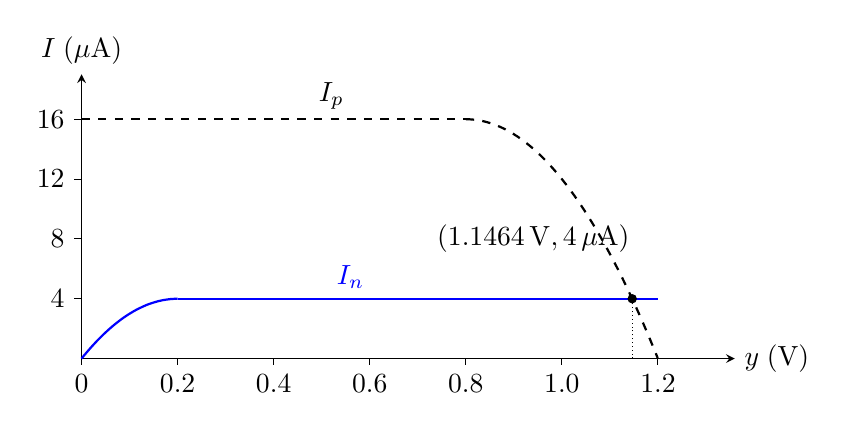
\begin{tikzpicture}[x=6.1cm,y=0.19cm,>=stealth]
\draw[->] (0,0)--(1.36,0) node[right] {\(y\;(\mathrm{V})\)};
\draw[->] (0,0)--(0,19) node[above] {\(I\;(\mu\mathrm{A})\)};
\foreach \x in {0,0.2,0.4,0.6,0.8,1.0,1.2}
 {\draw (\x,0)--(\x,-0.4) node[below] {\(\x\)};}
\foreach \y in {4,8,12,16}
 {\draw (0,\y)--(-0.015,\y) node[left] {\(\y\)};}
\draw[thick,blue,domain=0:0.2,samples=40]
 plot (\x,{200*(0.2*\x-\x*\x/2)});
\draw[thick,blue] (0.2,4)--(1.2,4);
\draw[thick,dashed] (0,16)--(0.8,16);
\draw[thick,dashed,domain=0.8:1.2,samples=45]
 plot (\x,{200*(0.4*(1.2-\x)-(1.2-\x)^2/2)});
\draw[densely dotted] (1.146410,0)--(1.146410,4);
\fill (1.146410,4) circle[radius=1.7pt];
\node[blue,above] at (0.56,4) {\(I_n\)};
\node[above] at (0.52,16) {\(I_p\)};
\node[anchor=west] at (0.72,8) {\((1.1464\,\mathrm{V},4\,\mu\mathrm{A})\)};
\end{tikzpicture}
\end{latin}
\caption{تقاطع جریان‌ها برای یک ورودی فرضی در مدل مربعی متقارن.
ساخت نمودار بر اساس روش شکل \secnum{۲.۲۶} کتاب است.}
\label{fig:inverter-current-intersection}
\end{figure}

جهت تغییر خروجی را نیز می‌توان از همین شکل فهمید. اگر در این
مثال \(y\) از مقدار تعادل کمتر شود، \(I_p>I_n\) و ظرفیت خروجی
شارژ می‌شود. اگر خروجی از تعادل بالاتر برود، \(I_n>I_p\) و خروجی
تخلیه می‌شود. این استدلال، بازگشت خروجی به تعادل را در همسایگی
نقطه نشان می‌دهد. در حالت استثنایی که دو منحنی در بازه‌ای کاملاً
روی هم قرار گیرند، مدل ایده‌آل خروجی یکتا نمی‌دهد. ناحیه \lr{C}
همین حالت را دارد.

\subsubsection{استخراج تحلیلی پنج ناحیه}
\label{sec:inverter-five-regions}
در ادامه فرض‌های \eqref{eq:inverter-symmetry} برقرارند، پس
\(a=V_{\mathrm{in}}-V_t\) و
\(b=V_{DD}-V_{\mathrm{in}}-V_t\) هستند. ترتیب نام‌های
\lr{A} تا \lr{E} از جدول \secnum{۲.۳} کتاب و اسلاید ۷ گرفته
شده است \cite{weste,dcslides}. نام ناحیه مدار، ترکیب ناحیه کاری
دو افزاره را مشخص می‌کند.

\paragraph*{ناحیه \lr{A} و خروجی بالا}
برای \(0\le V_{\mathrm{in}}\le V_t\)، ترانزیستور \lr{nMOS}
در مدل ایده‌آل جریان صفر دارد. چون \(V_{DD}>2V_t\)، ترانزیستور
\lr{pMOS} روشن است. شرط \lr{KCL}، جریان آن را نیز صفر می‌کند.
در شاخه \lr{Linear}، معادله جریان آن چنین است
\[
 0=\beta(bu-u^2/2)=\beta u(b-u/2).
\]
دو جواب جبری \(u=0\) و \(u=2b\) به دست می‌آیند. شرط
\(0\le u<b\) فقط \(u=0\) را می‌پذیرد. بنابراین،
\begin{equation}
 \boxed{V_{\mathrm{out}}=V_{DD},\qquad I_{DD}=0}.
 \label{eq:inverter-region-a}
\end{equation}
ترانزیستور روشن می‌تواند در حالت ماندگار جریان صفر داشته باشد.
اینجا اختلاف ولتاژ سورس و درین \lr{pMOS} صفر شده است. مسیر
هدایت آن، هنگام جابه‌جایی خروجی، بار لازم را فراهم کرده است.

\paragraph*{ناحیه \lr{B} و کاهش اولیه خروجی}
برای \(V_t<V_{\mathrm{in}}<V_{DD}/2\)، ابتدا فرض می‌کنیم
\lr{nMOS} در اشباع و \lr{pMOS} در \lr{Linear} است.
در این بازه \(0<a<b\) داریم. برابری جریان‌ها می‌دهد
\begin{align}
 \frac{\beta a^2}{2}&=\beta(bu-u^2/2),\notag\\
 a^2&=2bu-u^2,\notag\\
 u^2-2bu+a^2&=0,\notag\\
 (u-b)^2&=b^2-a^2.
 \label{eq:inverter-b-quadratic}
\end{align}
در مرحله دوم، تقسیم بر \(\beta>0\) و ضرب در دو انجام شده است.
تمام جمله‌های سه سطر آخر واحد \(\unit{\volt\squared}\) دارند.
با ریشه‌گرفتن، دو پاسخ جبری حاصل می‌شوند.
\[
 u=b\pm\sqrt{b^2-a^2}.
\]
ریشه با علامت مثبت از \(b\) بزرگ‌تر است و شرط \lr{Linear}
برای \lr{pMOS} را نقض می‌کند. ریشه مجاز و خروجی متناظر عبارت‌اند از
\begin{align}
 u&=b-\sqrt{b^2-a^2},\notag\\
 \boxed{V_{\mathrm{out}}=V_{DD}-b+\sqrt{b^2-a^2}}.
 \label{eq:inverter-b-root}
\end{align}
چون \(0<a<b\)، مقدار رادیکال بین صفر و \(b\) است.
پس \(0<u<b\) و \lr{pMOS} واقعاً در \lr{Linear} است.
همچنین \(V_{DD}-b=V_{\mathrm{in}}+V_t\)، پس
ترتیب ولتاژها چنین است.
\[
 V_{\mathrm{out}}>V_{\mathrm{in}}+V_t>V_{\mathrm{in}}-V_t=a.
\]
شرط اشباع \lr{nMOS} نیز برقرار است.
خروجی از تغذیه کمتر است، زیرا \(u>0\).

برای نوشتن خروجی فقط برحسب ورودی، اتحاد تفاضل دو مربع را به کار
می‌بریم. چون \(b-a=V_{DD}-2V_{\mathrm{in}}\) و
\(b+a=V_{DD}-2V_t\)، داریم
\begin{equation}
 \boxed{V_{\mathrm{out}}=V_{\mathrm{in}}+V_t+
 \sqrt{(V_{DD}-2V_{\mathrm{in}})(V_{DD}-2V_t)}}.
 \label{eq:inverter-b-transfer}
\end{equation}
هر دو عامل زیر رادیکال در این بازه مثبت‌اند. ریشه حاصل واحد ولت
دارد. تفاضل دو عدد نزدیک ممکن است در محاسبه عددی، دقت را کم کند.
برای بازنویسی پایدارتر افت ولتاژ نزدیک خروجی بالا، صورت و مخرج را
در مزدوج ضرب می‌کنیم
\[
 b-\sqrt{b^2-a^2}
 =\frac{(b-\sqrt{b^2-a^2})(b+\sqrt{b^2-a^2})}
        {b+\sqrt{b^2-a^2}}
 =\frac{a^2}{b+\sqrt{b^2-a^2}}.
\]
در مرحله آخر، اتحاد تفاضل دو مربع، صورت را به
\(b^2-(b^2-a^2)=a^2\) تبدیل کرده است. بنابراین، برای محاسبه داریم
\begin{equation}
 u=\frac{a^2}{b+\sqrt{b^2-a^2}},\qquad
 V_{\mathrm{out}}=V_{DD}-u.
 \label{eq:inverter-b-stable}
\end{equation}
مخرج مثبت است. با نزدیک‌شدن ورودی به \(V_t\) از بالا،
\(a\to0\)، \(u\to0\) و خروجی به \(V_{DD}\) می‌رسد.
با نزدیک‌شدن ورودی به \(V_{DD}/2\) از پایین،
خروجی به \(V_{DD}/2+V_t\) می‌رسد.

\paragraph*{ناحیه \lr{C} و اشباع هم‌زمان}
وقتی هر دو افزاره در اشباع‌اند، شرط جریان می‌شود
\begin{equation}
 \frac{\beta}{2}(V_{\mathrm{in}}-V_t)^2
 =\frac{\beta}{2}(V_{DD}-V_{\mathrm{in}}-V_t)^2.
 \label{eq:inverter-c-current-equality}
\end{equation}
اضافه‌ولتاژهای دو طرف مثبت‌اند، پس برابرشدن مربع‌ها در این دامنه
به برابری خود اضافه‌ولتاژها می‌انجامد. بنابراین،
\(V_{\mathrm{in}}-V_t=V_{DD}-V_{\mathrm{in}}-V_t\) و در نتیجه
\begin{equation}
 \boxed{V_{\mathrm{in}}=\frac{V_{DD}}{2}}.
 \label{eq:inverter-c-input}
\end{equation}
شرط اشباع \lr{nMOS}، \(V_{\mathrm{out}}\ge V_{DD}/2-V_t\) و
شرط اشباع \lr{pMOS}، \(V_{\mathrm{out}}\le V_{DD}/2+V_t\) است.
پس تمام خروجی‌های بازه زیر معادله ماندگار مدل را برآورده می‌کنند
\begin{equation}
 \boxed{\frac{V_{DD}}{2}-V_t\le V_{\mathrm{out}}
              \le\frac{V_{DD}}{2}+V_t},\qquad
 I_{DD}=\frac{\beta}{2}\left(\frac{V_{DD}}{2}-V_t\right)^2.
 \label{eq:inverter-c-output-interval}
\end{equation}
جریان ایده‌آل اشباع به خروجی وابسته نیست، پس معادله جریان در این
بازه ابزار تعیین خروجی یکتا ندارد. مقدار بار اولیه یا اثرهای
کنارگذاشته‌شده می‌توانند در تعیین خروجی نقش داشته باشند.
روی نمودار، این مجموعه یک پاره‌خط عمودی در
\(V_{\mathrm{in}}=V_{DD}/2\) است. توصیف شیب منفی بی‌نهایت در
کتاب، حد گذار بسیار تند را بیان می‌کند
\cite[صفحه ۸۸]{weste}. در خود مدل ایده‌آل، شیب تابع تک‌مقداری
در این پاره‌خط تعریف نمی‌شود.

\paragraph*{ناحیه \lr{D} و نزدیک‌شدن خروجی به زمین}
برای \(V_{DD}/2<V_{\mathrm{in}}<V_{DD}-V_t\)، فرض می‌کنیم
\lr{nMOS} در \lr{Linear} و \lr{pMOS} در اشباع است.
اینجا \(0<b<a\) داریم و شرط جریان چنین می‌شود
\begin{align}
 \beta(ay-y^2/2)&=\frac{\beta b^2}{2},\notag\\
 y^2-2ay+b^2&=0,\notag\\
 (y-a)^2&=a^2-b^2,\notag\\
 y&=a\pm\sqrt{a^2-b^2}.
 \label{eq:inverter-d-quadratic}
\end{align}
ریشه مثبت از \(a\) بزرگ‌تر است و شرط \lr{Linear} افزاره پایین
را نقض می‌کند. ریشه مجاز برابر است با
\begin{equation}
 \boxed{V_{\mathrm{out}}=a-\sqrt{a^2-b^2}}
 =\frac{b^2}{a+\sqrt{a^2-b^2}}.
 \label{eq:inverter-d-root}
\end{equation}
چون \(0<b<a\)، داریم \(0<y<a\) و شرط \lr{Linear} برقرار است.
همچنین \(y<a=V_{\mathrm{in}}-V_t<
V_{\mathrm{in}}+V_t\)، پس شرط اشباع \lr{pMOS} نیز برقرار است.
با جای‌گذاری \(a-b=2V_{\mathrm{in}}-V_{DD}\) و
\(a+b=V_{DD}-2V_t\)، خروجی برحسب ورودی نوشته می‌شود
\begin{equation}
 \boxed{V_{\mathrm{out}}=V_{\mathrm{in}}-V_t-
 \sqrt{(2V_{\mathrm{in}}-V_{DD})(V_{DD}-2V_t)}}.
 \label{eq:inverter-d-transfer}
\end{equation}
با نزدیک‌شدن ورودی به نقطه میانی از بالا، خروجی به
\(V_{DD}/2-V_t\) می‌رسد. در حد
\(V_{\mathrm{in}}\to V_{DD}-V_t\) از پایین،
\(b\to0\) و خروجی به صفر می‌رسد.

\paragraph*{ناحیه \lr{E} و خروجی پایین}
برای \(V_{DD}-V_t\le V_{\mathrm{in}}\le V_{DD}\)،
\lr{pMOS} در مدل ایده‌آل خاموش و \lr{nMOS} روشن است.
از \lr{KCL}، جریان \lr{nMOS} هم صفر می‌شود.
معادله \(0=\beta y(a-y/2)\) ریشه‌های \(y=0\) و \(y=2a\)
را می‌دهد. شرط \(0\le y<a\)، ریشه صفر را می‌پذیرد. پس
\begin{equation}
 \boxed{V_{\mathrm{out}}=0,\qquad I_{DD}=0}.
 \label{eq:inverter-region-e}
\end{equation}
در این حالت، \lr{nMOS} روشن و اختلاف ولتاژ درین و سورس آن صفر
است. با تغییر کوچک خروجی از زمین، مسیر پایین‌کش می‌تواند بار را
تخلیه کند.

\subsubsection{مشخصه انتقال، جریان تغذیه و مثال عددی}
\label{sec:inverter-transfer-example}
جدول \ref{tab:inverter-five-regions} نتیجه استخراج را با ترتیب
مرجع جمع می‌کند. در مرز بین دو شاخه، می‌توان از هر رابطه‌ای که
شرط مرزی را پوشش می‌دهد استفاده کرد، زیرا جریان‌ها پیوسته‌اند.
در مدل ایده‌آل، مجموعه خروجی‌های \lr{C} بازه مشخصی دارد.
\begin{table}[!htbp]
\centering
\small
\caption{پنج ناحیه مدار برای آستانه‌ها و \(\beta\)های برابر.
فرض \(V_{DD}>2V_t\) برقرار است.}
\label{tab:inverter-five-regions}
\begin{tabular}{cccl}
\toprule
ناحیه & \lr{nMOS} & \lr{pMOS} & شرط ورودی\\
\midrule
\lr{A} & \lr{Cutoff} & \lr{Linear} & \(0\le V_{\mathrm{in}}\le V_t\)\\
\lr{B} & \lr{Saturation} & \lr{Linear} & \(V_t<V_{\mathrm{in}}<V_{DD}/2\)\\
\lr{C} & \lr{Saturation} & \lr{Saturation} & \(V_{\mathrm{in}}=V_{DD}/2\)\\
\lr{D} & \lr{Linear} & \lr{Saturation} & \(V_{DD}/2<V_{\mathrm{in}}<V_{DD}-V_t\)\\
\lr{E} & \lr{Linear} & \lr{Cutoff} & \(V_{DD}-V_t\le V_{\mathrm{in}}\le V_{DD}\)\\
\bottomrule
\end{tabular}
\end{table}

شکل \ref{fig:inverter-ideal-vtc} مشخصه مدل را با نسبت فرضی
\(\tau=V_t/V_{DD}=0.25\) رسم می‌کند. محورهای نرمال‌شده
\(x=V_{\mathrm{in}}/V_{DD}\) و \(z=V_{\mathrm{out}}/V_{DD}\)
بی‌بعدند. از روابط \eqref{eq:inverter-b-transfer} و
\eqref{eq:inverter-d-transfer}، دو شاخه میانی چنین می‌شوند
\begin{equation}
 z_B=x+\tau+\sqrt{(1-2x)(1-2\tau)},\qquad
 z_D=x-\tau-\sqrt{(2x-1)(1-2\tau)}.
 \label{eq:inverter-normalized-vtc}
\end{equation}
در این نمودار، گذار عمودی از \(z=0.75\) تا \(z=0.25\) است.
خروجی در دو سوی این گذار با شاخه‌های رادیکالی تغییر می‌کند.
\begin{figure}[!htbp]
\centering
\begin{latin}
\PersianMathDigits
\begin{tikzpicture}[x=7.3cm,y=4.6cm,>=stealth]
\draw[->] (0,0)--(1.12,0) node[right] {\(V_{\mathrm{in}}/V_{DD}\)};
\draw[->] (0,0)--(0,1.13) node[above] {\(V_{\mathrm{out}}/V_{DD}\)};
\foreach \x in {0.25,0.5,0.75,1.0}
 {\draw (\x,0)--(\x,-0.02) node[below] {\(\x\)};}
\foreach \y in {0.25,0.5,0.75,1.0}
 {\draw (0,\y)--(-0.013,\y) node[left] {\(\y\)};}
\draw[densely dotted] (0,0)--(1,1);
\draw[densely dotted] (0.25,0)--(0.25,1);
\draw[densely dotted] (0.75,0)--(0.75,0.2);
\draw[thick,blue] (0,1)--(0.25,1);
\draw[thick,blue,domain=0.25:0.5,samples=90]
 plot (\x,{\x+0.25+sqrt(max(0,(1-2*\x)*0.5))});
\draw[thick,blue] (0.5,0.75)--(0.5,0.25);
\draw[thick,blue,domain=0.5:0.75,samples=90]
 plot (\x,{\x-0.25-sqrt(max(0,(2*\x-1)*0.5))});
\draw[thick,blue] (0.75,0)--(1,0);
\fill (0.5,0.5) circle[radius=1.6pt];
\node at (0.12,0.9) {A};
\node at (0.36,0.85) {B};
\node[right] at (0.51,0.62) {C};
\node at (0.64,0.15) {D};
\node at (0.9,0.1) {E};
\node[anchor=west] at (0.64,0.57) {\(V_{\mathrm{inv}}/V_{DD}=0.5\)};
\end{tikzpicture}
\end{latin}
\caption{مشخصه انتقال محاسبه‌شده برای مدل متقارن و
\(V_t/V_{DD}=0.25\). خط نقطه‌چین مورب، شرط
\(V_{\mathrm{out}}=V_{\mathrm{in}}\) را نمایش می‌دهد.}
\label{fig:inverter-ideal-vtc}
\end{figure}

در بازه روشن‌بودن هر دو افزاره، جریان مدار از افزاره اشباع‌شده
به دست می‌آید. با تعریف \(A_0=V_{DD}/2-V_t>0\)، نتیجه چنین است
\begin{equation}
 I_{DD}=
 \begin{cases}
 0,&0\le V_{\mathrm{in}}\le V_t,\\[2pt]
 \dfrac{\beta}{2}(V_{\mathrm{in}}-V_t)^2,
     &V_t<V_{\mathrm{in}}\le V_{DD}/2,\\[4pt]
 \dfrac{\beta}{2}(V_{DD}-V_{\mathrm{in}}-V_t)^2,
     &V_{DD}/2<V_{\mathrm{in}}<V_{DD}-V_t,\\[4pt]
 0,&V_{DD}-V_t\le V_{\mathrm{in}}\le V_{DD}.
 \end{cases}
 \label{eq:inverter-supply-current}
\end{equation}
بیشینه جریان این مدل در ورودی میانی برابر
\(I_{DD,\max}=\beta A_0^2/2\) است. شکل
\ref{fig:inverter-supply-current} جریان نرمال‌شده را رسم می‌کند.
\begin{figure}[!htbp]
\centering
\begin{latin}
\PersianMathDigits
\begin{tikzpicture}[x=7.3cm,y=3.3cm,>=stealth]
\draw[->] (0,0)--(1.12,0) node[right] {\(V_{\mathrm{in}}/V_{DD}\)};
\draw[->] (0,0)--(0,1.18) node[above] {\(I_{DD}/I_{DD,\max}\)};
\foreach \x in {0.25,0.5,0.75,1.0}
 {\draw (\x,0)--(\x,-0.025) node[below] {\(\x\)};}
\draw (0,1)--(-0.013,1) node[left] {\(1\)};
\draw[thick,blue] (0,0)--(0.25,0);
\draw[thick,blue,domain=0.25:0.5,samples=45] plot (\x,{16*(\x-0.25)^2});
\draw[thick,blue,domain=0.5:0.75,samples=45] plot (\x,{16*(0.75-\x)^2});
\draw[thick,blue] (0.75,0)--(1,0);
\draw[densely dotted] (0.5,0)--(0.5,1)--(0,1);
\end{tikzpicture}
\end{latin}
\caption{جریان تغذیه مدل مربعی برای نسبت آستانه
\(V_t/V_{DD}=0.25\)، مطابق رابطه \eqref{eq:inverter-supply-current}.
محورها بی‌بعدند.}
\label{fig:inverter-supply-current}
\end{figure}

اگر ورودی در یک مقدار میانی ثابت نگه داشته شود، این جریان در
مدل \lr{DC} به‌طور پیوسته وجود دارد. اگر ورودی از زمین به تغذیه
گذار کند، برای مدتی از بازه هدایت هم‌زمان عبور می‌کند. کتاب این
عبور را با یک پالس جریان توضیح می‌دهد
\cite[شکل \secnum{۲.۲۶} و صفحه ۸۸]{weste}.
شکل جریان برحسب ورودی، زمان و پهنای پالس را تعیین نمی‌کند.
محاسبه جریان طی گذار، به سرعت تغییر ورودی و دینامیک خروجی نیاز دارد.
در ورودی‌های نزدیک دو ریل، جریان ایده‌آل صفر می‌شود. در افزاره
واقعی، نشتی‌های آموزش‌داده‌شده در جزوه دوم وجود دارند.

\paragraph*{محاسبه کامل یک نقطه در \lr{B}}
پارامترهای فرضی شکل \ref{fig:inverter-current-intersection} را
به کار ببرید. در \(V_{\mathrm{in}}=\qty{0.5}{\volt}\)،
\(a=\qty{0.2}{\volt}\) و \(b=\qty{0.4}{\volt}\) است.
از \eqref{eq:inverter-b-root}، افت ولتاژ \lr{pMOS} برابر است با
\begin{equation}
 u=0.4-\sqrt{0.4^2-0.2^2}
   =0.4-\sqrt{0.12}\approx\qty{0.05359}{\volt},\qquad
 y\approx\qty{1.14641}{\volt}.
 \label{eq:inverter-b-numerical}
\end{equation}
ریشه دیگر، \(u\approx\qty{0.74641}{\volt}\)، شرط
\(u<b=\qty{0.4}{\volt}\) را نقض می‌کند. برای ریشه مجاز،
\(y>\qty{0.2}{\volt}\) و \(u<\qty{0.4}{\volt}\) هستند.
پس \lr{nMOS} در اشباع و \lr{pMOS} در \lr{Linear} است.
محاسبه دو جریان به‌صورت مستقل می‌دهد
\begin{align}
 I_n&=(200/2)(0.2)^2=\qty{4.000}{\micro\ampere},\notag\\
 I_p&=200[0.4(0.0535898)-(0.0535898)^2/2]
       \approx\qty{4.000}{\micro\ampere}.
 \label{eq:inverter-b-current-check}
\end{align}
در سطرهای عددی، ضریب جریان برحسب
\(\unit{\micro\ampere\per\volt\squared}\) و ولتاژها برحسب ولت
جای‌گذاری شده‌اند. توان دریافت‌شده از تغذیه در این نقطه چنین است.
\[
 P=V_{DD}I_{DD}=1.2(4)=\qty{4.8}{\micro\watt}.
\]

\paragraph*{محاسبه کامل یک نقطه در \lr{D}}
در همان مدار، اگر \(V_{\mathrm{in}}=\qty{0.7}{\volt}\)،
\(a=\qty{0.4}{\volt}\) و \(b=\qty{0.2}{\volt}\) می‌شود.
از \eqref{eq:inverter-d-root}، خروجی به دست می‌آید.
\[
 y=0.4-\sqrt{0.4^2-0.2^2}\approx\qty{0.05359}{\volt}.
\]
ریشه بزرگ‌تر \(y\approx\qty{0.74641}{\volt}\) از
\(a=\qty{0.4}{\volt}\) بیشتر است و شرط \lr{Linear}
برای \lr{nMOS} را نقض می‌کند. برای ریشه مجاز،
\(y<a\) و \(u=1.2-y\approx\qty{1.14641}{\volt}>b\) هستند.
پس \lr{nMOS} در \lr{Linear} و \lr{pMOS} در اشباع است.
دو جریان برابر \(\qty{4}{\micro\ampere}\) و توان نیز
\(\qty{4.8}{\micro\watt}\) است.

جدول \ref{tab:inverter-numerical-transfer} چند نقطه دیگر را نشان
می‌دهد. به‌دلیل تقارن، خروجی‌ها در دو ورودی مکمل به‌صورت
\(y(V_{DD}-v)=V_{DD}-y(v)\) مرتبط‌اند. در ورودی میانی،
\(y\in[\qty{0.3}{\volt},\qty{0.9}{\volt}]\) و جریان
\(\qty{9}{\micro\ampere}\) است. توان ماندگار آن نقطه در مدل
ایده‌آل \(\qty{10.8}{\micro\watt}\) می‌شود.
\begin{table}[!htbp]
\centering
\small
\caption{نمونه‌های محاسبه‌شده برای پارامترهای فرضی
\(V_{DD}=\qty{1.2}{\volt}\)، \(V_t=\qty{0.3}{\volt}\) و
\(\beta=\qty{200}{\micro\ampere\per\volt\squared}\).
اعداد تا رقم‌های نمایش‌داده‌شده گرد شده‌اند.}
\label{tab:inverter-numerical-transfer}
\begin{tabular}{cccc}
\toprule
\(V_{\mathrm{in}}\)، \(\unit{\volt}\) &
\(V_{\mathrm{out}}\)، \(\unit{\volt}\) &
\(I_{DD}\)، \(\unit{\micro\ampere}\) & ناحیه\\
\midrule
\num{0.00} & \num{1.2000} & \num{0} & \lr{A}\\
\num{0.30} & \num{1.2000} & \num{0} & مرز \lr{A/B}\\
\num{0.40} & \num{1.1899} & \num{1.00} & \lr{B}\\
\num{0.50} & \num{1.1464} & \num{4.00} & \lr{B}\\
\num{0.55} & \num{1.0949} & \num{6.25} & \lr{B}\\
\num{0.60} & بازه \(0.3\le y\le0.9\) & \num{9.00} & \lr{C}\\
\num{0.65} & \num{0.1051} & \num{6.25} & \lr{D}\\
\num{0.70} & \num{0.0536} & \num{4.00} & \lr{D}\\
\num{0.80} & \num{0.0101} & \num{1.00} & \lr{D}\\
\num{0.90} & \num{0.0000} & \num{0} & مرز \lr{D/E}\\
\num{1.20} & \num{0.0000} & \num{0} & \lr{E}\\
\bottomrule
\end{tabular}
\end{table}

\subsubsection{شیب مشخصه و اثر \lr{CLM}}
\label{sec:inverter-clm}
در مدل ایده‌آل، \(I_n\) و \(I_p\) در اشباع به ولتاژ خروجی
وابسته نیستند. \lr{CLM} این استقلال را تغییر می‌دهد و مقاومت
خروجی محدود ایجاد می‌کند. کتاب، همین اثر را علت شیب محدود و
گسترش ناحیه \lr{C} واقعی به بازه‌ای از ورودی‌ها می‌داند
\cite[صفحه ۸۸ و بخش \secnum{۲.۴.۲}]{weste}.

برای نمایش تحلیلی این نکته، تنها در دامنه اشباع هم‌زمان، مدل
مربعی با \lr{CLM} را به کار می‌بریم. تعریف کنید
\(N=\beta_na^2/2\) و \(P=\beta_pb^2/2\). این دو کمیت واحد
آمپر دارند. آنگاه با \(\lambda_n,\lambda_p>0\) داریم
\begin{equation}
 I_n=N(1+\lambda_n y),\qquad
 I_p=P[1+\lambda_p(V_{DD}-y)].
 \label{eq:inverter-clm-currents}
\end{equation}
عامل‌های داخل پرانتز بی‌بعدند و واحد \(\lambda\)،
\(\unit{\per\volt}\) است. برابری جریان‌ها به‌صورت خطی برحسب
خروجی حل می‌شود
\begin{align}
 N+N\lambda_n y&=P+P\lambda_pV_{DD}-P\lambda_p y,\notag\\
 (N\lambda_n+P\lambda_p)y&=P(1+\lambda_pV_{DD})-N,\notag\\
 \boxed{y=\frac{P(1+\lambda_pV_{DD})-N}
                    {N\lambda_n+P\lambda_p}}.
 \label{eq:inverter-clm-output}
\end{align}
صورت واحد آمپر و مخرج واحد آمپر بر ولت دارد، پس جواب ولتاژ است.
پس از حل باید \(a,b>0\) و
\(a\le y\le V_{\mathrm{in}}+V_{TP}\) بررسی شوند. این رابطه
فقط در محدوده‌ای که هر دو افزاره در اشباع‌اند معتبر است.
اگر یکی از شرط‌ها نقض شود، رابطه جریان همان افزاره باید عوض شود.

\paragraph*{مثال آموزشی خروجی یکتا در ناحیه میانی}
به پارامترهای فرضی قبلی،
\(\lambda_n=\lambda_p=\qty{0.1}{\per\volt}\) اضافه کنید.
در \(V_{\mathrm{in}}=\qty{0.6}{\volt}\)، داریم
\(a=b=\qty{0.3}{\volt}\) و \(N=P=\qty{9}{\micro\ampere}\).
رابطه \eqref{eq:inverter-clm-output} می‌دهد
\[
 y=\frac{9(1+0.1\times1.2)-9}{9(0.1)+9(0.1)}
 =\qty{0.6}{\volt}.
\]
هر دو شرط اشباع برقرارند، زیرا
\(\qty{0.3}{\volt}\le y\le\qty{0.9}{\volt}\).
جریان از رابطه مدل به دست می‌آید.
\[
 I_{DD}=9(1+0.1\times0.6)=\qty{9.54}{\micro\ampere}.
\]
جدول \ref{tab:inverter-clm-results} چند ورودی نزدیک را
نشان می‌دهد. همه ردیف‌های جدول، پس از کنترل ناحیه کاری پذیرفته
شده‌اند. اعداد، نتیجه مدل آموزشی‌اند.
\begin{table}[!htbp]
\centering
\caption{اثر \lr{CLM} در چند نقطه با اشباع هم‌زمان، برای
\(\lambda_n=\lambda_p=\qty{0.1}{\per\volt}\) و پارامترهای مثال.}
\label{tab:inverter-clm-results}
\begin{tabular}{ccc}
\toprule
\(V_{\mathrm{in}}\)، \(\unit{\volt}\) &
\(V_{\mathrm{out}}\)، \(\unit{\volt}\) &
\(I_{DD}\)، \(\unit{\micro\ampere}\)\\
\midrule
\num{0.596} & \num{0.8826} & \num{9.5349}\\
\num{0.598} & \num{0.7413} & \num{9.5387}\\
\num{0.600} & \num{0.6000} & \num{9.5400}\\
\num{0.602} & \num{0.4587} & \num{9.5387}\\
\num{0.604} & \num{0.3174} & \num{9.5349}\\
\bottomrule
\end{tabular}
\end{table}

برای نمونه، به‌کاربردن همین رابطه در
\(V_{\mathrm{in}}=\qty{0.595}{\volt}\)، خروجی
\(y\approx\qty{0.9532}{\volt}\) می‌دهد. اما حد اشباع
\lr{pMOS} در آن ورودی \(y\le\qty{0.895}{\volt}\) است.
پس این پاسخ با فرض اشباع هم‌زمان سازگار نیست و باید با ترکیب
\lr{Saturation/Linear} دوباره حل شود. قرارگرفتن عدد در بازه
زمین تا تغذیه به‌تنهایی برای پذیرش جواب کافی نیست.

\paragraph*{استخراج \lr{Gain} با تغییرهای کوچک}
برای یک تغییر کوچک ورودی و خروجی در نقطه اشباع هم‌زمان،
جریان \lr{nMOS} را به‌صورت زیر تغییر می‌دهیم
\begin{equation}
 \mathrm{d}I_n=g_{m,n}\,\mathrm{d}V_{\mathrm{in}}
                +g_{ds,n}\,\mathrm{d}y.
 \label{eq:inverter-small-change-n}
\end{equation}
در اینجا \(g_{m,n}>0\) نرخ تغییر جریان با گیت در خروجی ثابت و
\(g_{ds,n}>0\) نرخ تغییر آن با خروجی در ورودی ثابت است.
هر دو واحد \(\unit{\siemens}=\unit{\ampere\per\volt}\) دارند.
برای بزرگی جریان \lr{pMOS}، افزایش ورودی، \(V_{SG,p}\) را کم
می‌کند و افزایش خروجی، \(V_{SD,p}\) را کم می‌کند. بنابراین،
\begin{equation}
 \mathrm{d}I_p=-g_{m,p}\,\mathrm{d}V_{\mathrm{in}}
                 -g_{ds,p}\,\mathrm{d}y.
 \label{eq:inverter-small-change-p}
\end{equation}
کمیت‌های \(g_{m,p},g_{ds,p}\) نیز بزرگی‌های مثبت‌اند. با
قرارگرفتن هر دو حالت نزدیک در تعادل، باید
\(\mathrm{d}I_n=\mathrm{d}I_p\) باشد. با جمع جمله‌ها نتیجه می‌شود
\begin{equation}
 \boxed{\frac{\mathrm{d}V_{\mathrm{out}}}{\mathrm{d}V_{\mathrm{in}}}
 =-\frac{g_{m,n}+g_{m,p}}{g_{ds,n}+g_{ds,p}}}.
 \label{eq:inverter-gain}
\end{equation}
این استخراج تکمیلی، اثر مقاومت خروجی محدود بر شیب را روشن می‌کند.
در مدل \eqref{eq:inverter-clm-currents}، مشتق‌ها چنین‌اند
\begin{align}
 g_{m,n}&=\beta_na(1+\lambda_n y),&
 g_{ds,n}&=\lambda_nN,\notag\\
 g_{m,p}&=\beta_pb[1+\lambda_p(V_{DD}-y)],&
 g_{ds,p}&=\lambda_pP.
 \label{eq:inverter-clm-derivatives}
\end{align}
در مرکز مثال، رسانایی‌ها چنین‌اند.
\[
 \begin{aligned}
 g_{m,n}=g_{m,p}&=\qty{63.6}{\micro\siemens},\\
 g_{ds,n}=g_{ds,p}&=\qty{0.9}{\micro\siemens}.
 \end{aligned}
\]
پس شیب محلی از نسبت رسانایی‌ها به دست می‌آید.
\[
 -\frac{63.6+63.6}{0.9+0.9}\approx-70.67.
\]
تغییر ورودی \(\qty{1}{\milli\volt}\) در همسایگی مرکز، حدود
\(\qty{70.7}{\milli\volt}\) تغییر خروجی در جهت مخالف ایجاد
می‌کند. این برآورد، تقریب خطی محلی است.

با میل \(\lambda_n,\lambda_p\) به صفر، رسانایی خروجی مدل به
صفر می‌رود و بزرگی شیب افزایش می‌یابد. در حد کاملاً ایده‌آل،
همان گذار عمودی و بازه خروجی ناحیه \lr{C} بازیابی می‌شود.
کتاب در شکل \secnum{۲.۲۷}، نتیجه شبیه‌سازی یک نمونه فناوری
\(\qty{65}{\nano\metre}\) را نشان می‌دهد که \lr{pMOS} آن دو
برابر \lr{nMOS} عرض دارد. شکل مرجع، گذار تند با شیب محدود را
نمایش می‌دهد \cite[صفحه ۸۹]{weste}. پارامترهای عددی این جزوه
برای توضیح مدل فرض شده‌اند و به آن نمونه نسبت داده نمی‌شوند.

\subsubsection{آستانه ورودی \lr{Inverter} و وابستگی دمایی}
\label{sec:inverter-input-threshold}
کتاب نقطه تقاطع مشخصه انتقال با خط
\(V_{\mathrm{out}}=V_{\mathrm{in}}\) را
\lr{Input Threshold} یا \(V_{\mathrm{inv}}\) می‌نامد
\cite[صفحه ۸۹]{weste}. بنابراین، تعریف این ولتاژ چنین است
\begin{equation}
 V_{\mathrm{out}}=V_{\mathrm{in}}=V_{\mathrm{inv}}.
 \label{eq:inverter-threshold-definition}
\end{equation}
آستانه \(V_t\) پارامتر یک ترانزیستور است. آستانه
\(V_{\mathrm{inv}}\) با برابرشدن ولتاژ ورودی و خروجی کل مدار
تعریف می‌شود. مثلاً در مثال حاضر، \(V_t=\qty{0.3}{\volt}\) و
\(V_{\mathrm{inv}}=\qty{0.6}{\volt}\) هستند.

در مدل متقارن، نقطه \(V_{DD}/2\) هم در بازه خروجی
\eqref{eq:inverter-c-output-interval} قرار دارد و هم شرط
\eqref{eq:inverter-threshold-definition} را برقرار می‌کند. پس
\begin{equation}
 \boxed{V_{\mathrm{inv}}=V_{DD}/2}.
 \label{eq:inverter-symmetric-threshold}
\end{equation}
این تعریف، از میان خروجی‌های مجاز مدل ایده‌آل، محل تقاطع با خط
مورب را مشخص می‌کند. در مدل متقارن با \lr{CLM} یکسان نیز
\(N=P\) در مرکز و رابطه \eqref{eq:inverter-clm-output} همان
خروجی \(V_{DD}/2\) را می‌دهد.

کتاب بیان می‌کند که کاهش \lr{Mobility} و بزرگی آستانه با دما
برای هر دو نوع افزاره رخ می‌دهد و آستانه ورودی مدار معمولاً
حساسیت دمایی کمتری دارد \cite[صفحه ۸۹]{weste}. در فرض تقارن
کامل و تغذیه ثابت، اگر دو آستانه در هر دما برابر و دو
\(\beta\) نیز در هر دما برابر بمانند، رابطه
\eqref{eq:inverter-symmetric-threshold} دقیقاً حفظ می‌شود.
خود جریان‌ها همچنان می‌توانند به‌شدت با دما تغییر کنند.
در مدار واقعی، تفاوت تغییر پارامترهای دو نوع افزاره و تغییر
تغذیه می‌تواند نقطه تقاطع را جابه‌جا کند. نسبت‌های نابرابر
\(\beta\) موضوع بخش \secnum{۲.۵.۲} هستند.

\subsubsection{تمرین‌های تشریحی و کنترل تحلیل}
\label{sec:inverter-practice}
\paragraph*{تمرین آموزشی ۱ و بررسی شرط‌های \lr{pMOS}}
فرض کنید \(V_{DD}=\qty{1.2}{\volt}\)،
\(V_{\mathrm{in}}=\qty{0.5}{\volt}\)،
\(V_{\mathrm{out}}=\qty{1.1}{\volt}\) و
\(V_{tp}=-\qty{0.3}{\volt}\) باشند. ناحیه کاری \lr{pMOS}
را با هر دو قرارداد ولتاژ تعیین کنید.

\textbf{پاسخ.}
در قرارداد مثبت، اختلاف ولتاژها چنین‌اند.
\[
 \begin{aligned}
 V_{SG,p}&=1.2-0.5=\qty{0.7}{\volt},\\
 V_{SD,p}&=1.2-1.1=\qty{0.1}{\volt}.
 \end{aligned}
\]
اضافه‌ولتاژ \(0.7-0.3=\qty{0.4}{\volt}\) و شرط
\(0.1<0.4\) برقرار است، پس افزاره در \lr{Linear} است.
در قرارداد علامت‌دار، \(V_{GS,p}=-\qty{0.7}{\volt}<V_{tp}\)
و \(V_{DS,p}=-\qty{0.1}{\volt}\) هستند.
شرط \(V_{DS,p}>V_{GS,p}-V_{tp}\) یعنی
نامساوی زیر نیز برقرار است.
\[
 -0.1>-0.7-(-0.3)=-0.4.
\]
برای ادعای تعادل کل مدار، باید جریان \lr{nMOS} و \lr{pMOS}
هم بررسی شوند. تعیین ناحیه یک افزاره، تعادل کل مدار را ثابت نمی‌کند.

\paragraph*{تمرین آموزشی ۲ و تشخیص ریشه فیزیکی}
در مدار متقارن مثال، برای ورودی \(\qty{0.7}{\volt}\)،
شخصی خروجی \(\qty{0.7464}{\volt}\) را از معادله درجه دوم
گزارش می‌کند. این جواب را بررسی کنید.

\textbf{پاسخ.}
در فرض ناحیه \lr{D}، باید \lr{nMOS} در \lr{Linear} باشد، یعنی
\(y<V_{\mathrm{in}}-V_t=\qty{0.4}{\volt}\).
ریشه گزارش‌شده این شرط را نقض می‌کند.
ریشه \(\qty{0.05359}{\volt}\) از \eqref{eq:inverter-d-root}
هم شرط \lr{nMOS} و هم شرط اشباع \lr{pMOS} را برآورده می‌کند.
پس باید همین ریشه انتخاب شود. هر دو ریشه معادله جبری را حل
می‌کنند، اما معادله با فرض یک ناحیه خاص استخراج شده است.

\paragraph*{تمرین آموزشی ۳ و مقیاس‌کردن جریان}
در مدل متقارن، هر دو \(\beta\) را دو برابر کنید و آستانه، تغذیه
و فرض بار \lr{DC} را ثابت نگه دارید. مشخصه انتقال و جریان چه
تغییری می‌کنند؟

\textbf{پاسخ.}
در \(I_n=I_p\)، ضریب مشترک دو از دو طرف حذف می‌شود، پس همان
خروجی‌ها به دست می‌آیند. در \(V_{\mathrm{in}}=\qty{0.5}{\volt}\)،
خروجی همچنان \(\qty{1.1464}{\volt}\) است، اما جریان از
\(\qty{4}{\micro\ampere}\) به \(\qty{8}{\micro\ampere}\)
می‌رسد. توان ماندگار این نقطه نیز از
\(\qty{4.8}{\micro\watt}\) به \(\qty{9.6}{\micro\watt}\)
می‌رسد. برای زمان گذار، تغییر ظرفیت ناشی از تغییر ابعاد نیز باید
در مدل دینامیکی وارد شود.

\paragraph*{تمرین آموزشی ۴ و ولتاژ میانی ایده‌آل}
در ورودی \(\qty{0.6}{\volt}\) مثال ایده‌آل، خروجی‌های
\(\qty{0.4}{\volt}\) و \(\qty{0.8}{\volt}\) را آزمایش کنید.
آیا هر دو می‌توانند شرط \lr{DC} مدل را برقرار کنند؟

\textbf{پاسخ.}
در هر دو حالت، اضافه‌ولتاژهای \(a=b=\qty{0.3}{\volt}\)
هستند. خروجی اول، \(y=\qty{0.4}{\volt}\ge a\) و
\(u=\qty{0.8}{\volt}\ge b\) می‌دهد. خروجی دوم،
\(y=\qty{0.8}{\volt}\ge a\) و
\(u=\qty{0.4}{\volt}\ge b\) می‌دهد.
پس هر دو افزاره در هر دو حالت اشباع‌اند و جریان‌ها
\(\qty{9}{\micro\ampere}\) هستند. هر دو خروجی در مدل ایده‌آل
تعادل دارند. با مدل \lr{CLM} متقارن مثال، حل یکتای مرکزی
\(\qty{0.6}{\volt}\) به دست می‌آید.

\paragraph*{مرور روش حل}
ابتدا ولتاژ سورس، گیت، درین و بدنه را بنویسید. قرارداد آستانه
\lr{pMOS} را مشخص کنید. جریان بار و فرض حالت ماندگار را تعیین
کنید. سپس اضافه‌ولتاژها و ترکیب ناحیه کاری را بنویسید، جریان‌ها
را برابر بگذارید و معادله را حل کنید. هر ریشه باید با شرط‌های
ناحیه کاری، بازه زمین تا تغذیه و واحدها کنترل شود. در نقطه میانی
مدل ایده‌آل، بازه خروجی را نگه دارید. برای مدل واقعی‌تر، اثرهای
غیرایده‌آل را با قرارداد یکسان و پارامترهای مشخص وارد کنید.
